% THEORETICAL FRAMEWORK

\cleardoublepage

\chapter{Theoretical framework}
\label{theoretical-framework}

\section{Problem Definition}
\label{problem-definition}
The problem of image registration is an optimization problem, and its candidate solutions are all the possible transformations that maximize or, equivalently, minimize a chosen (di)similarity measure that quantifies the image similarity between the fixed and moving image; poses as the target function.

Depending on the particular problem setting (e.g. deformable registration), we will either face a linear or nonlinear optimization problem, which will affect the possible solution strategies.

\section{Mono and Multi-modal Image Registration}
\label{mono-multimodal-registration}

\section{Rigid and Non-rigid Registration}
\label{image-a}
The rigid registration setting, the resulting transformation is expressed as a matrix mapping each point of the moving image to the target / fixed image. The possible transformations expressed by the matrix are rigid and affine transformations. Rigid transformations are limited to rotations and translations, and affine transformations extend the rigid setting, allowing for stretching and skewing.

In the non-rigid case, limitations are lifted, and allows for arbitrary mappings of individual image pixels, producing displacement fields. 

The problem with displacement fields is that, depending on the setting, only a subset of all possible transformations are indeed plausible, so the definition is extended to accomodate for this. A particular deformation is said to be plausible if the pixel movement is smooth, simulating natural elastic deformation.

Usually, regularization techniques are employed in order to enforce the aforementioned properties.

\section{Image Warping}
\label{image-warping}

\section{Diffeomorphism}
\label{Diffeomorphism}

\section{Classical Methods}
\label{classical-methods}
Demons, other iterative methods...

\section{Deep learning-based methods}
\label{deep-learning-methods}
When approaching the original problem of image registration... When using deep learning, we don't directly calculate the 


Differences between unsupervised and supervised deep learning methods.

\subsection{U-Net}
\label{u-net}
Some paper of implementation using U-Net or similar model

\section{Transformers}
\label{transformers}
Transformers were introduced ...

Currently, state of the art in sequence processing, tasks such as NLP...

Encoder vs Decoder.



\subsection{Mechanism of Self-attention}
\label{self-attention}

When using transformers, the input sequence is tokenized, obtaining a set of tokens - a collection of distinct, unordeded elements.


The next step is the projection of the tokens into a distributed geometrical space of continuous-valued vectors - what is referred to as an embedding. This is done in order to preserve the semantical relationships among the tokens.

In this low-dimensional space, we expect that the projections of the original tokens which hold stronger semantic relationships with each other are, indeed, closer to each other than their counterparts.


However, after the tokenization step, we have effectively lost the order of the original sequence. In order to maintain the notion of order necessary to process the input as a sequence,
transformer blocks use positional encoding.

Positional encoding alters the embeddings depending of the position of the token in the original sequence.

One of the possible techniques for implementing positional encoding is using the sinousoidal function. 

We then perform feature-based attention on the resulting embeddings.
The inductive bias by which feature-based attention is based upon, is to allow the network to place its attention not only based
in the original order of the sequence, but taking into account the content of the tokens.

In order to quantify the similarity of tokens, we will calculate the vector similarity among the tokens' projections
into the learned embedding space. As this is a low-dimensional space, we can make use of the inner vector product.

The transformer uses 3 different representations of the embedding matrix, the queries, keys and values.

For each token (i.e. vector), we create a query vector, key vector and value vector. The query, key and value matrices are
learned as part of the training process.
In order to reduce the computational complexity of the operation, this resulting vectors are usually in lower-dimensional spaces.

The concepts of key, value and query are originally part of information retrieval systems.


Self attention is performed for each position.

The main idea is that we compute the similarity of each token of the sequence with each other token. Then, the result of the 
self-attention is a vector, result of the sum of each token in the sequence multiplied by its similarity score. In this
way, we are capturing the most important context individually for each of the tokens in the sequence.


Self-attention with matrices
First, we obtain the query, key and value matrices by multiplying the embedding matrix with the learned weight matrices WQ, WK, WV.
Each of the rows of the embedding matrix corresponds to a token of the input sequence.

$$softmax(\frac{Q K^T}{\sqrt{d_k}}) V = Z$$

The softmax outputs a probability distribution, with all of its components adding to one.

This concept of self-attention is further developed with multi-headed attention.

\subsection{Encoder Block}
\label{encoder-block}

\subsection{Decoder Block}
\label{decoder-block}

\subsection{Multi-head Self-attention}
\label{multihead-self-attention}

With multi-headed attention, we repeat the original self-attention process, obtaining multiple representational spaces, in the form of 
multiple sets of query, key and value matrices. Theoretically, this allows the model to perform attention in different, independent low-dimensional spaces, which
translates to the ability to jointly perform attention from different representation subspaces, at different positions.

\section{Vision Transformers}
\label{vision-transformers}

In \cite{Dosovitskiy2021-be}, vision transformers are introduced.

- Parallelizable
- Bigger receptive fields compared to CNN

\begin{figure}
    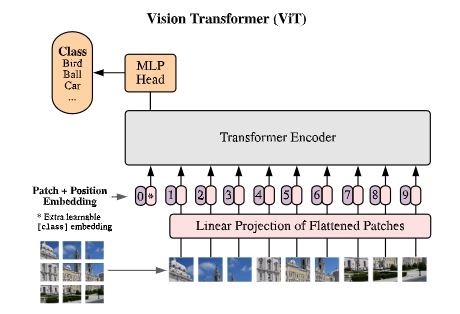
\includegraphics{vision-transformer-diagram}
    \caption{Diagram of Vision Transformer. Adapted from \citenum{Dosovitskiy2021-be}}
    \label{fig:vision-transformer-diagram}
\end{figure}

In order for a transformer network to be able to handle 2D images, they propose a method to convert 2D images into sequences by splitting the original image into smaller 2D patches, which are then further processed as described in \ref{encoder-block}.

Formally, the original image $x \in \mathbb{R}^{H \times W \times C}$ is reshaped into a sequence of flattened 2D patches $x_p \in \mathbb{R}^{N \times P^2 \cdot C}$, where $(H,W)$ is the original resolution of the image, $C$ denotes the number of channels, $(P,P)$ is the patch resolution, and $N=HW/P^2$ is the total patch number (i.e. sequence length).

Also, the paper explores the possibility of feature maps obtained from a CNN as the input sequence, as an alternative to the aforementioned image patches.

In terms of the positional embeddings, they employ 1D positional embeddings. They also tried using 2D positional encodings without showing any further improvements in the model's performance.

One of the most important discoveries of the paper is that, upon inspection, the attention distance (i.e. average distance in image space across which information is integrated), analogous to the receptive field size of CNNs, is far greater than in its counterpart. 

\begin{figure}[h!]
    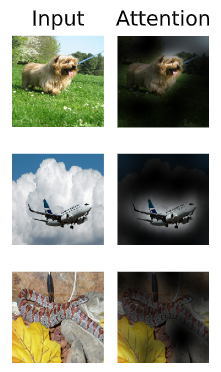
\includegraphics[width=1.0\textwidth]{image-self-attention}
    \caption{Visualization of Self-Attention on Input Images. Reproduced from \citenum{Dosovitskiy2021-be}}
    \label{fig:image-self-attention}
\end{figure}

The results empirically confirm that the ability of performing of global attention, enabled by the self-attention mechanism, is used by the model in practice, where some of the attention heads attend most of the image already in the lower layers.

\section{SymTrans}
\label{symtrans}

\subsection{Convolution-based Efficient Multi-head Self-attention (CEMSA)}
\label{cemsa-block}
Due to the large number of parameters of transformer blocks...

Depth-wise separable and grouped convolution.

$$x^{q,k,v}=Flatten(Conv3D(Reshape(x),s))$$,
where $x$ is the input token to the CEMSA block.

The positional embedding is removed, in order to further reduce the total parameters.

Depth-wise separable convolutional operations are used in order to capture the local features of the input images, and also compress memory and parameters.

\begin{figure}
    \centering
    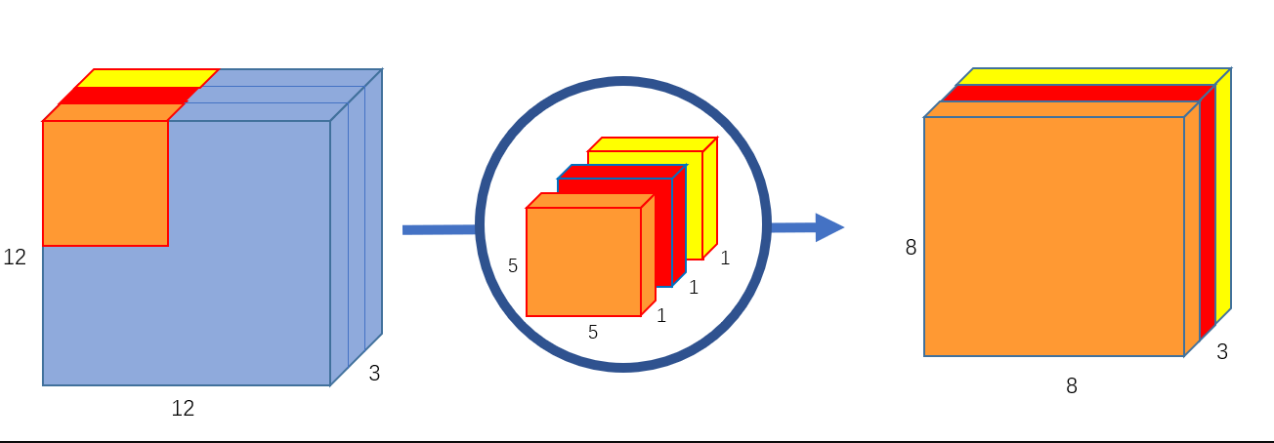
\includegraphics[width=1.0\textwidth]{depthwise-convolution}
    \caption{Visualization of Depth-wise Convolution. Reproduced from \citenum{Wang2018-ks}}
    \label{fig:depthwise-convolution}
\end{figure}

Depth-wise convolution is applied by using a single convolutional filter for each input channel. After convolving each input channel with its filter, the resulting feature maps are stacked along the dimension axis. 

depthwise convolution applies a single convolutional filter per each input channel and pointwise convolution is used to create a linear combination of the output of the depthwise convolution. https://paperswithcode.com/method/depthwise-separable-convolution

The grouped convolution is 1/g of the filters is applied to each 1/g of the input

The grouped convolution is employed to reduce the parameters before the linear projections, in a magnitude of $1/g$.

In \cite{Dosovitskiy2021-be}, it is already mentioned that replacing image patches with feature maps obtained from a CNN is a possibility.

\begin{figure}
    \centering
    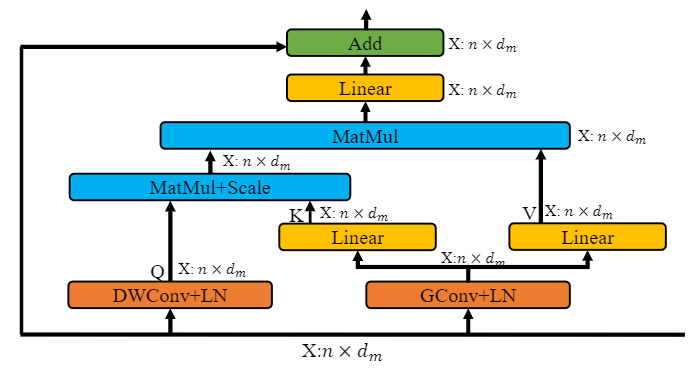
\includegraphics[width=1.0\textwidth]{cemsa-block}
    \caption{Visualization of CEMSA block. Reproduced from \citenum{Mingrui_Ma2022-ug}}
    \label{fig:cemsa-block}
\end{figure}

Spatial-reduction ratio that reduces the size of image via Conv. (sr-ratio)

\begin{figure}
    \centering
    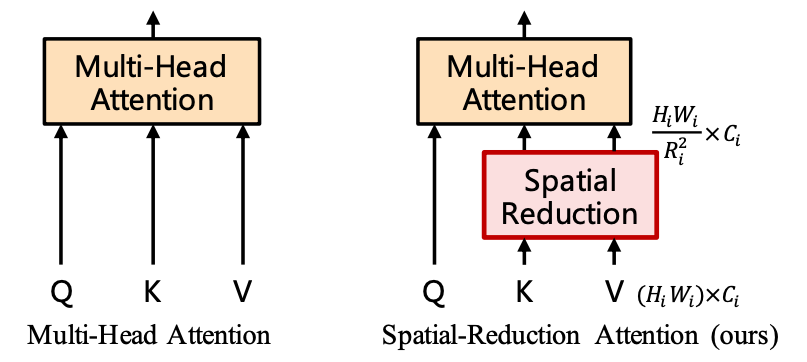
\includegraphics[width=1.0\textwidth]{spatial-reduction}
    \caption{Comparison of Multi-Head Attention and Spatial Reduction Attention. Reproduced from \citenum{Wang2021-kw}}
    \label{fig:spatial-reduction-attention}
\end{figure}

Spatial Reduction Attention
Reduces the spatial scale of the key and value before the attention operation, in order to reduce the computational and memory overhead of the operation.

https://paperswithcode.com/method/spatial-reduction-attention

DropPath is dropping an entire sample from the batch, which effectively results in stochastic depth when used as in Eq. 2 of their paper. On the other hand, Dropout is dropping random values, as expected (from the docs):

Stochastic depth mentioned in \cite{Huang2016-np}

https://www.youtube.com/watch?v=fEVyfT-gLqQ


Permutation equivariant transformer thanks to attention mechanism.

TODO: Still don't fully understand decoder part

Spatial Transformer Networks \cite{Jaderberg2015-kg}
The idea behind standard transformer blocks is to make the network spatially invariant, seeking the disentanglement of object pose and part deformation from texture and shape.

Stationary Velocity Field, scaling and squaring approach

